\documentclass[pdf]{beamer}
\usepackage[utf8]{inputenc}
\usepackage[czech]{babel}
\usepackage{graphics}

\setbeamertemplate{footline}[frame number]


\begin{document}

\begin{frame}
  \begin{center}
    
\includegraphics[scale=0.13]{app_menu_header}
  \end{center}
\end{frame}

\begin{frame}{Tým}
  \begin{minipage}{\textwidth}
    \textbf{Brno Erasmus Guide}
    \begin{enumerate}
      \item Android    
      \item přehled fakult, menz, kolejí a akcí
      \item data offline
    \end{enumerate}
    \vspace{2\baselineskip}
  \end{minipage}
  \begin{minipage}{\textwidth}
    \begin{itemize}
      \item Jakub Fišer (Projektový manažer) - design a UX (45\%)
      \item Jan Duda (Vývojář) - fb připojení, seznamy, detaily (45\%)
      \item Norbert Fábián (Zákazník) - accommodation activita, image loading, jsony (10\%)
    \end{itemize}  
  \end{minipage}
\end{frame}

\begin{frame}{Co naše aplikace obsahuje}  
 %Jak jsme to tvorili, popis implementovane cinnosti.
 \begin{itemize}
   \item seznamy fakult, kantýn a ubytoven - načítány z internetu
   \item zobrazení základních informací o fakultě, kantýně nebo ubytovně
   \item zobrazení polohy dané budovy na mapě
   \item offline uchování seznamů všech budov po prvním načtení
   \item agregace eventů z facebooku
 \end{itemize}  
\end{frame}

\begin{frame}{Komplikace}
 %Jakym technickym problemum jsme celili a jak jsme je vyresili.
 \begin{itemize}
   \item poměr stran obrázků - PercentRelativeLayout
   \item logika navigace - Activity vs. Fragment
   \item omezení FB SDK - ID skupiny
   \item ikona - bitmapové vs. vektorové nástroje
 \end{itemize}
\end{frame}

\begin{frame}{Screenshoty}
  \begin{center}
    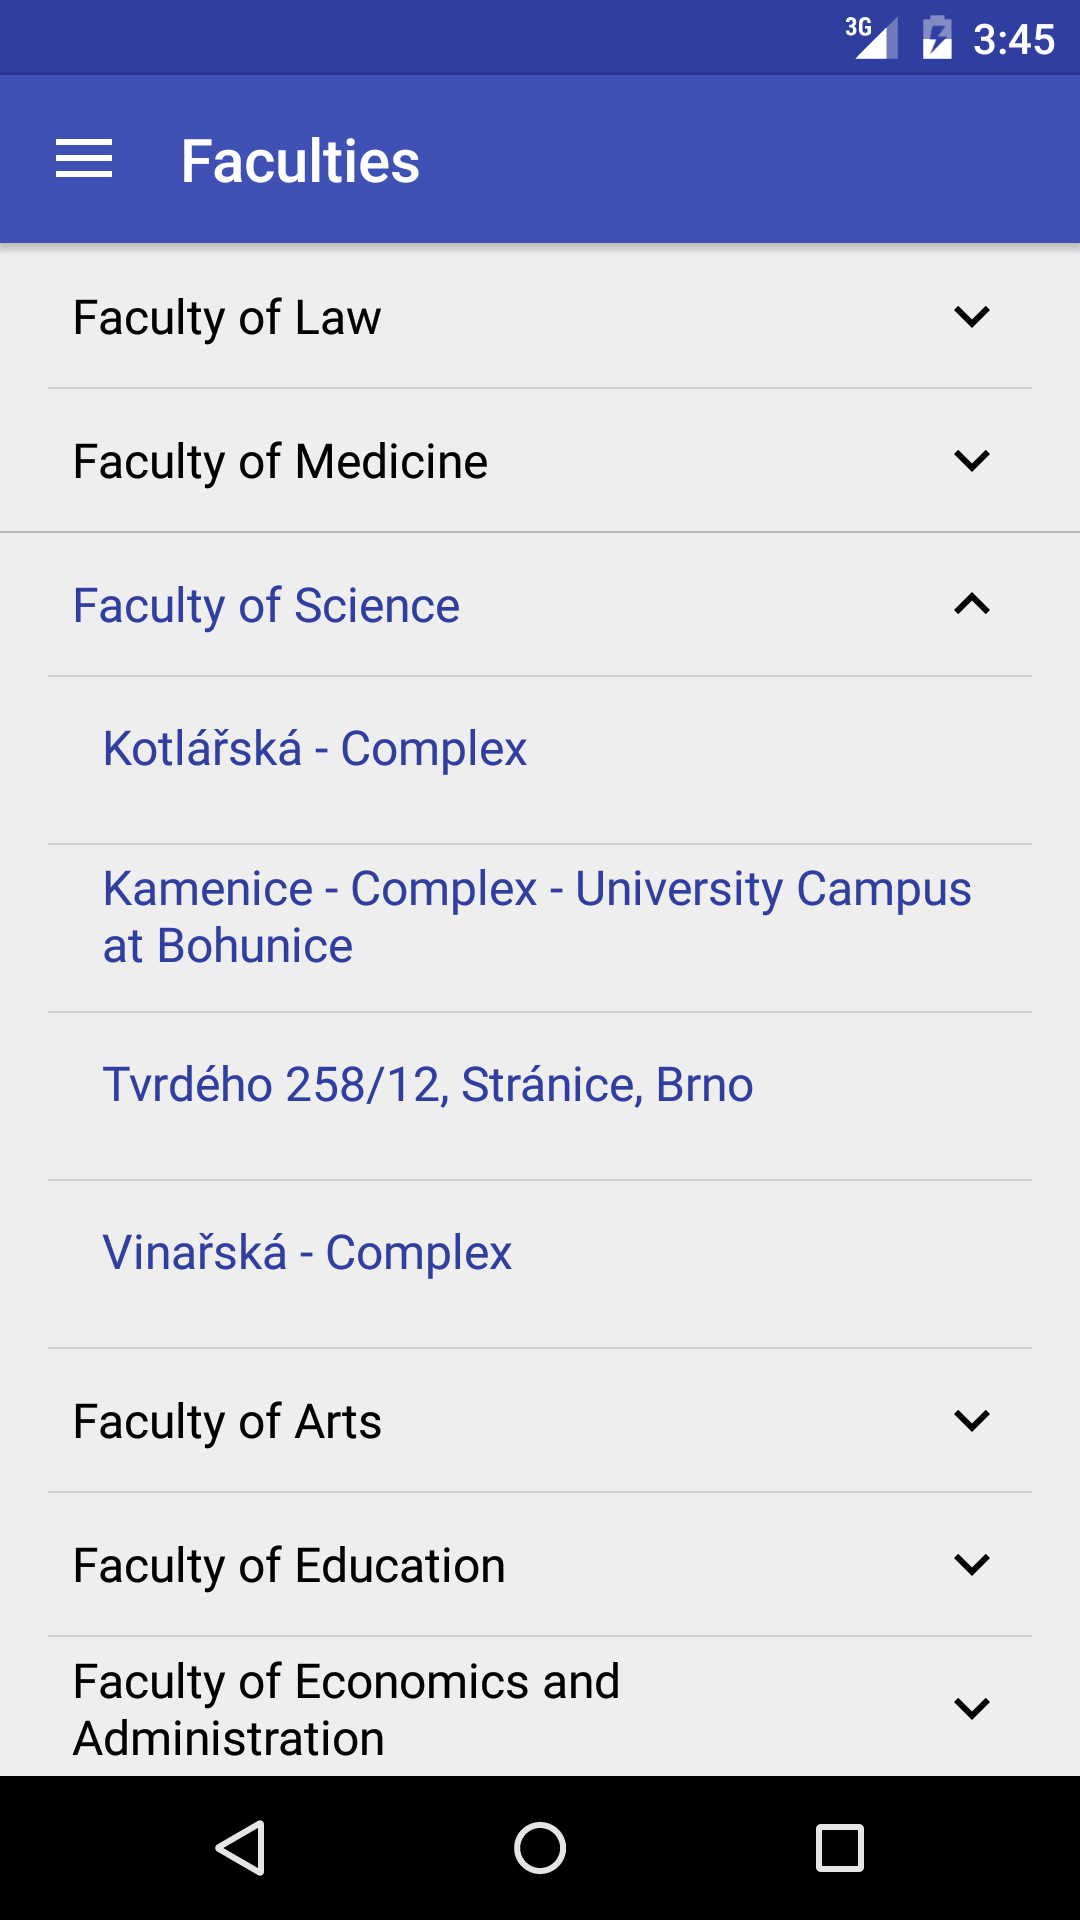
\includegraphics[scale=0.1]{app-list}
    \hspace{10px}
    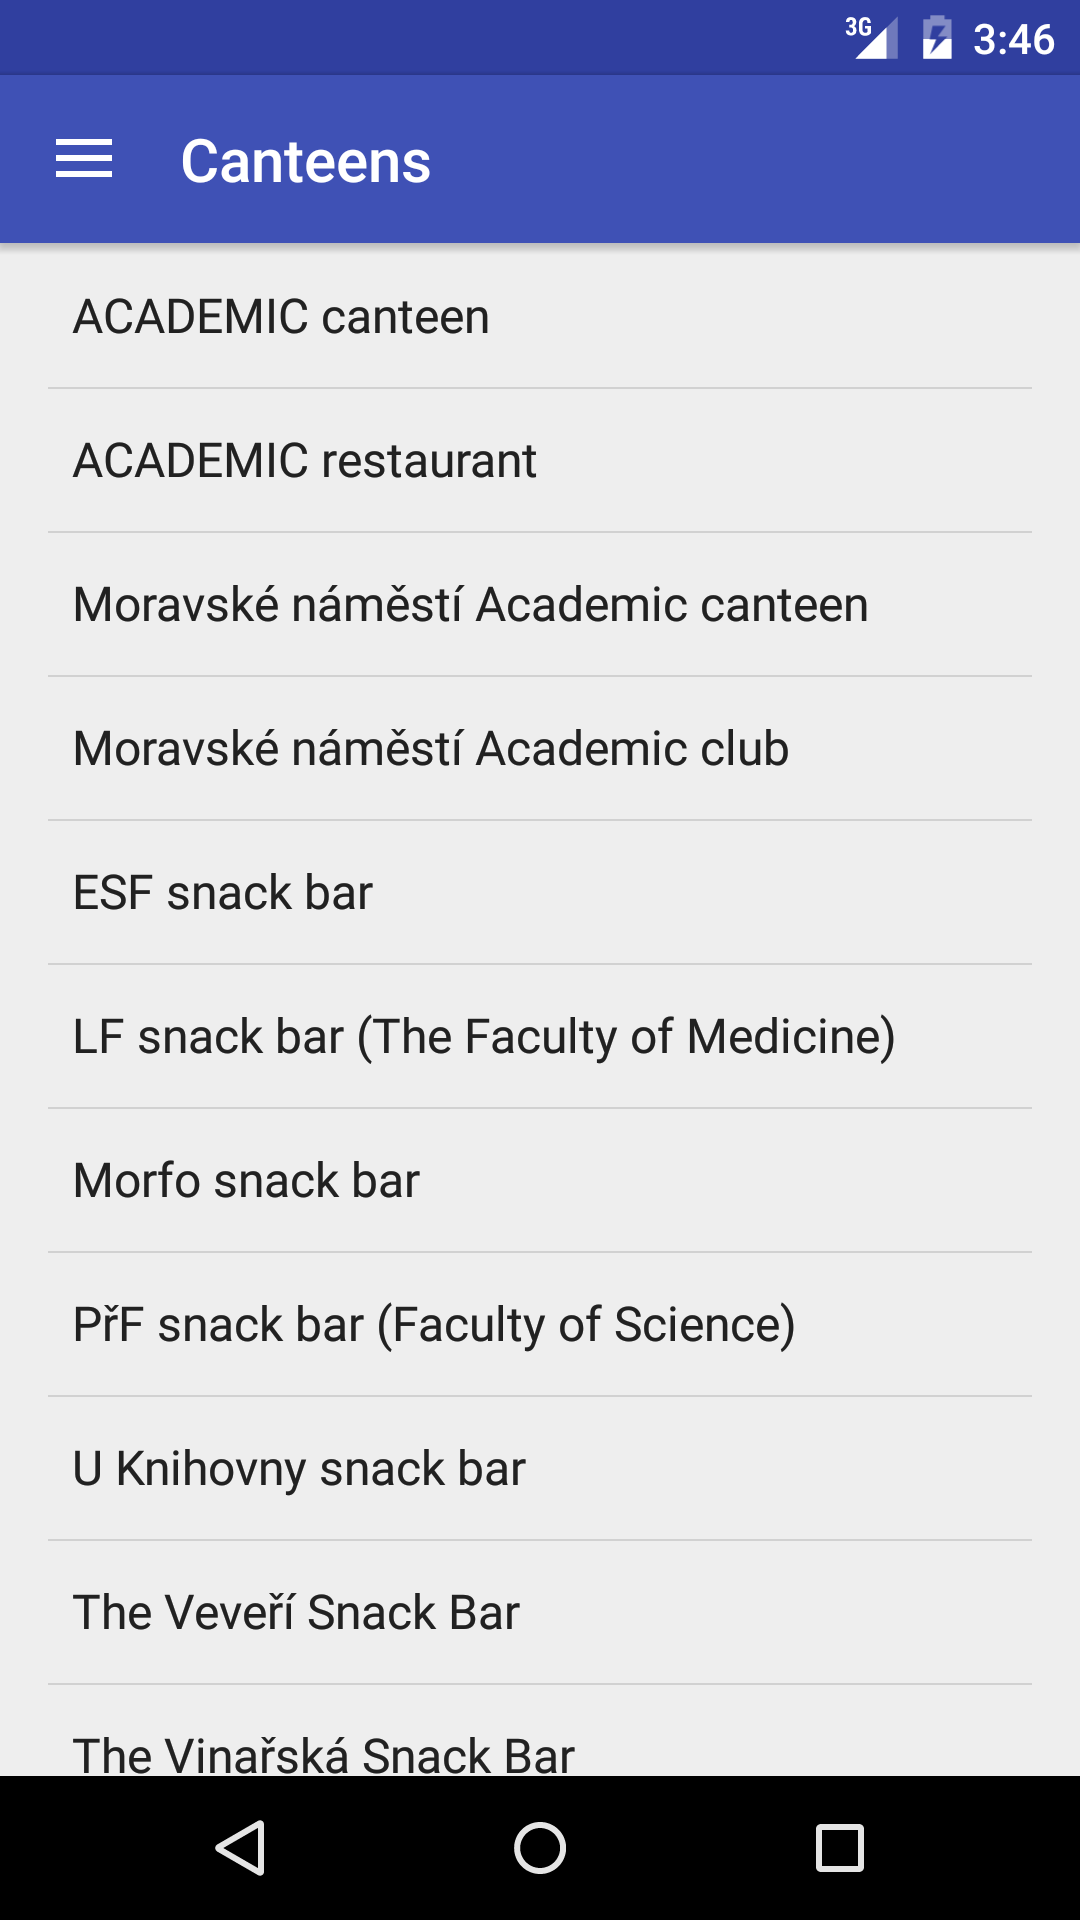
\includegraphics[scale=0.1]{app-list2}
  \end{center}
\end{frame}

\begin{frame}{Screenshoty}
  \begin{center}
    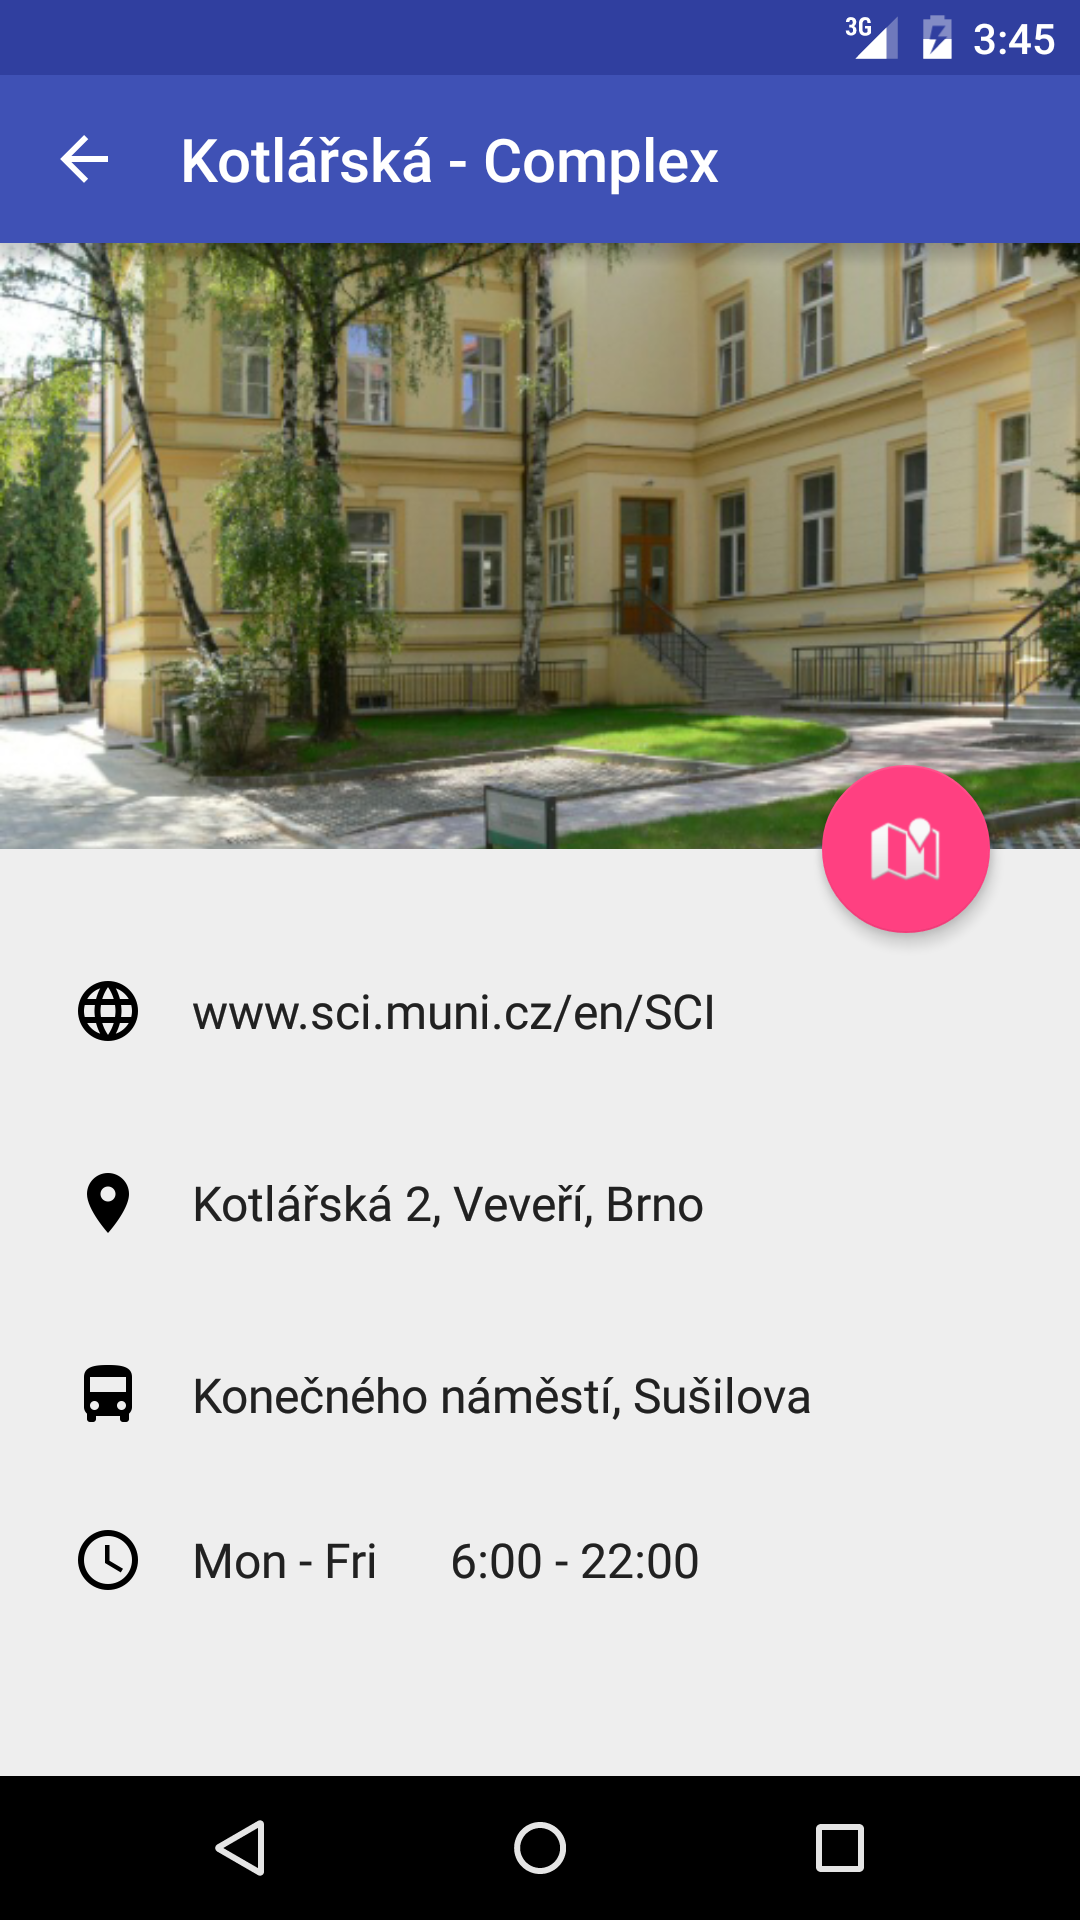
\includegraphics[scale=0.1]{app-detail}
    \hspace{10px}
    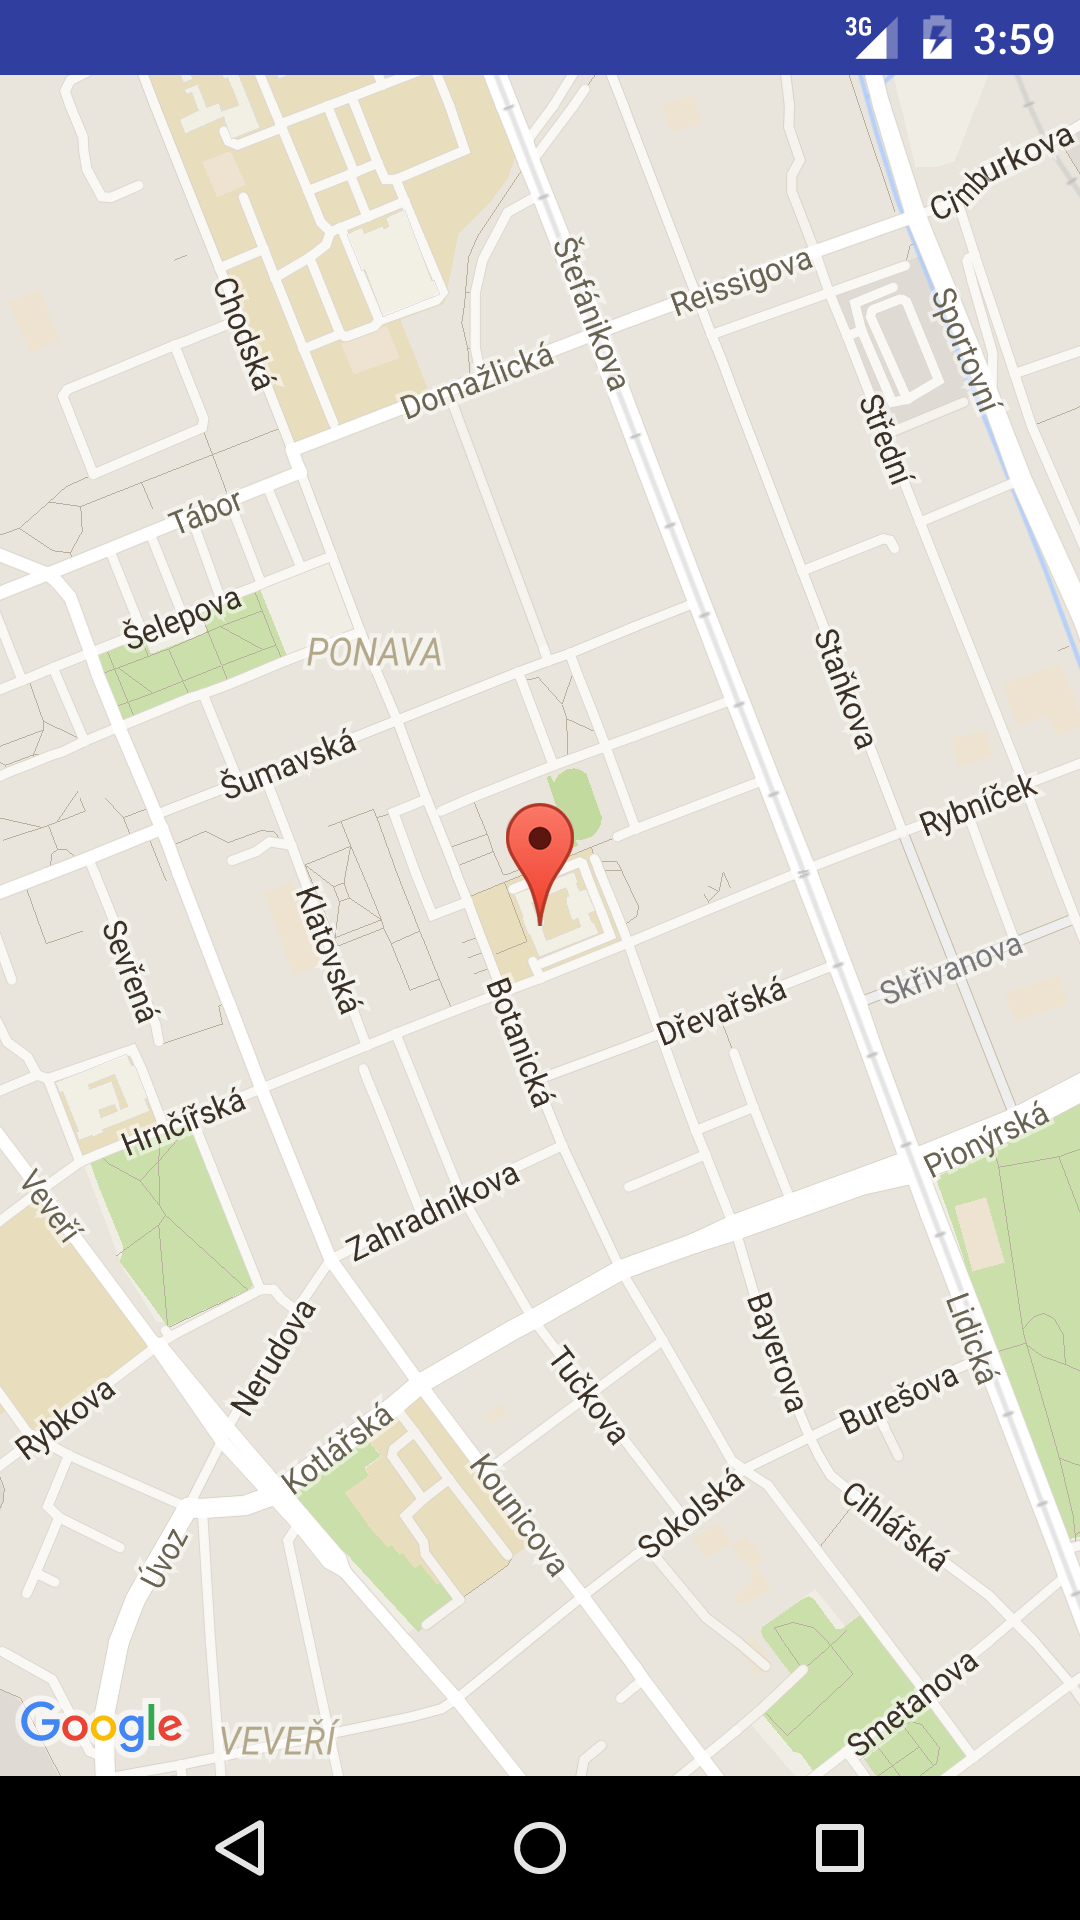
\includegraphics[scale=0.1]{app-map}
  \end{center}
\end{frame}

\begin{frame}{Screenshoty}
  \begin{center}
    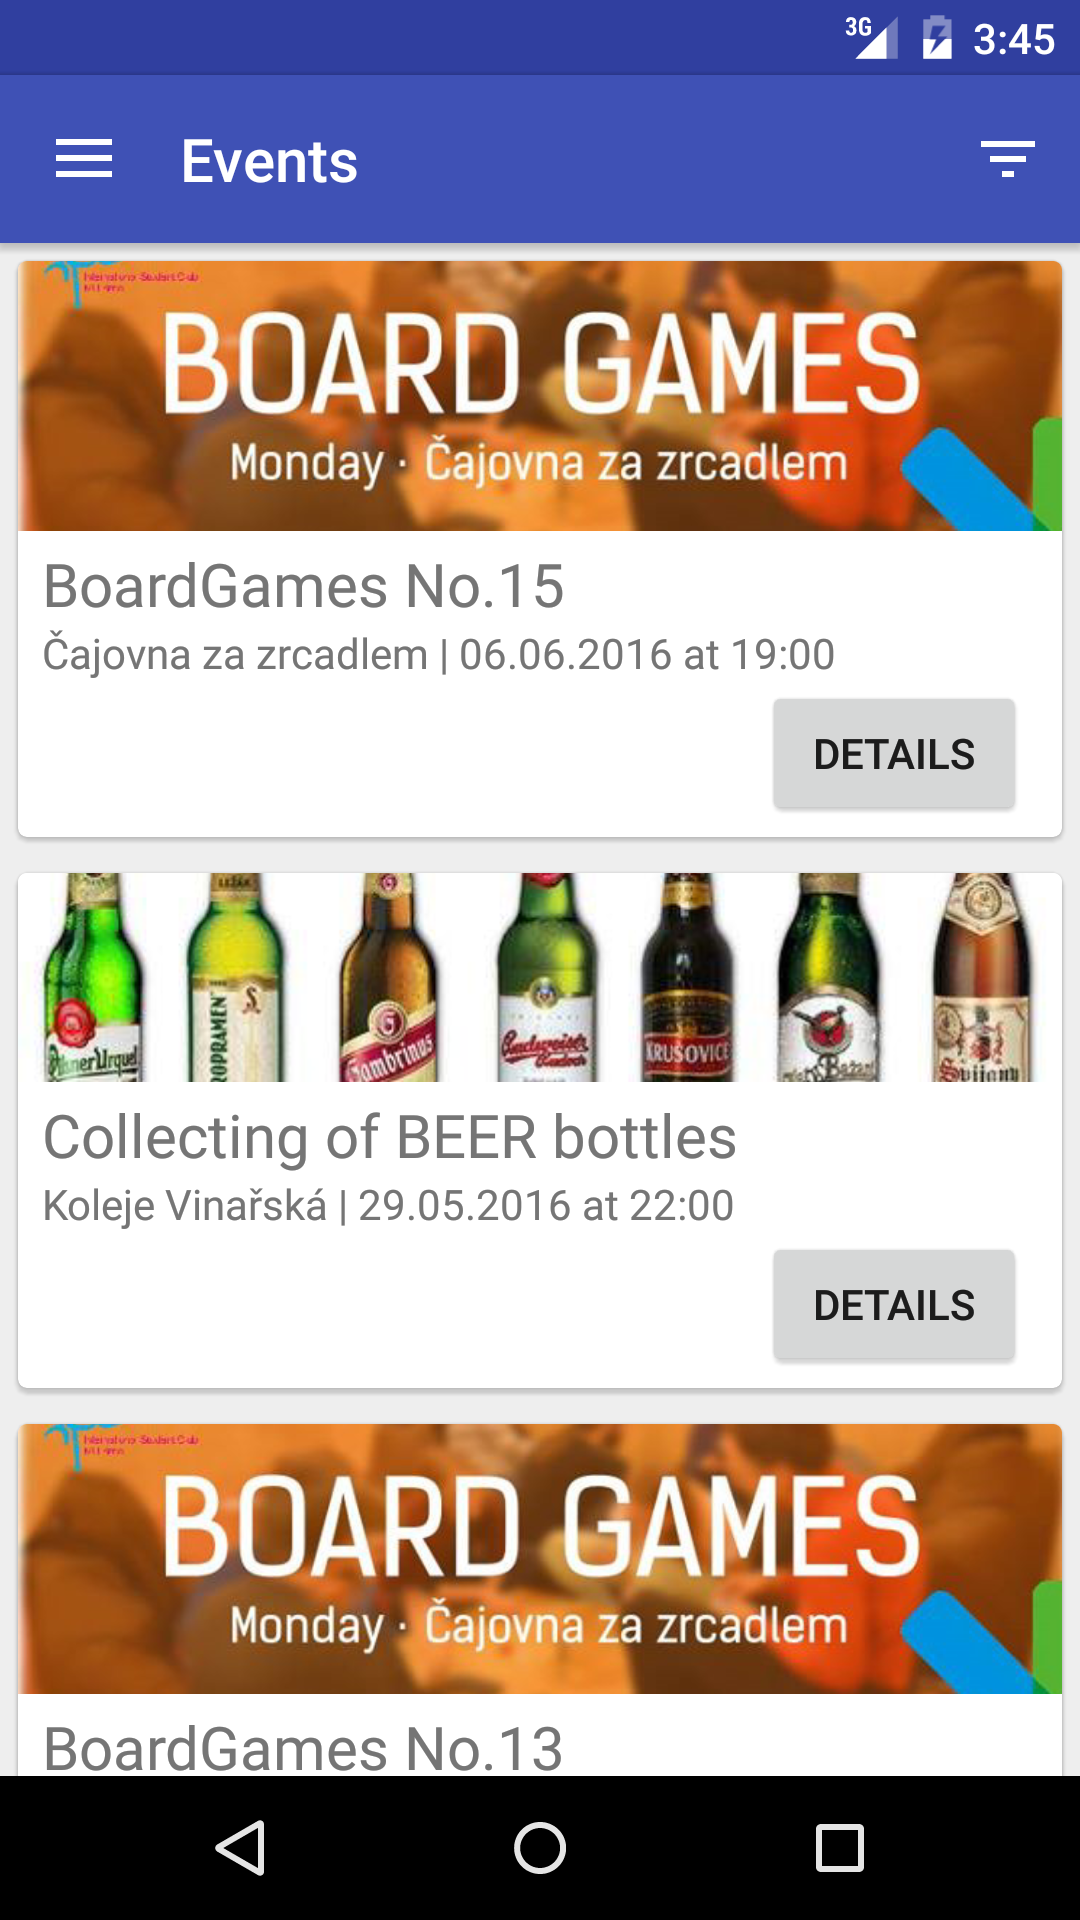
\includegraphics[scale=0.1]{app-event}
  \end{center}
\end{frame}

\end{document}